\documentclass[12pt,twocolumn]{article}
\usepackage[T1]{fontenc}
\usepackage{graphicx}
\usepackage{amsmath}
\usepackage[left=1cm,right=1cm,top=2cm,bottom=2cm]{geometry}
%\renewcommand*{\familydefault}{\sfdefault}
\title{\vspace{-2.5em}Investigation 2: 1D Diffusion}
\author{Christopher Pattison}
\date{}
\begin{document}
\maketitle
\section*{Non-Linear Diffusion}
\[
\nabla\cdot k \nabla T = q
\]
The heat equation is solved where \emph{k} is a function of \emph{T}. The equation is discretized with the Finite
Volume Method with \emph{k} varying in space
\[\int_V\frac{dkdT}{dx^2} + q = 0\]
\[k\left.\frac{dT}{dx}\right\rvert_{x_w}^{x_e} + q(x_e-x_w)\]
\[\Delta x_e=x_E-x_P;\hspace{1em} \Delta x_w=x_P-x_W\]
\[\frac{k_e (T_E-T_P)}{\Delta x_e} - \frac{k_w (T_P-T_W)}{\Delta x_w} + q\Delta x\]
\[\frac{k_e}{\Delta x_e} T_E - (\frac{k_e}{\Delta x_e} + \frac{k_w}{\Delta x_w})T_P + \frac{k_w}{\Delta x_w} T_W + q(x_e-x_w)\]
When some \emph{k(T)} is plugged in, a non-linear system is obtained that can be solved by a non-linear solver.
\[k(T) = k_0 + k_1 e^{-\frac{T}{T_0}}\]
\[k_e = \frac{2}{k(T_E)^{-1}+k(T_P)^{-1}} ;\hspace{1em} k_w = \frac{2}{k(T_P)^{-1}+k(T_W)^{-1}}\]
\section*{Non-Linear Solvers}
\subsection*{Picard Iteration}
Picard Iteration involves selecting an initial guess for \emph{T} then iteratively reforming \emph{A} and solving for \emph{T}.
Because it fails to acknowledge much of a relationship (other than its existence) between \emph{T} and its coefficients, it
performs extremely slow for strongly non-linear systems.
\[A_nx_{n+1} = b\]
If a non-linear model is to be used for \emph{b}, it is also just a matter of updating \emph{b} every iteration.
\subsection*{Newton's Method}
Newton's Method solves for the zeros of a function. We can define a vector valued residual function
\[R = Ax-b\]
Since \emph{R} = \textbf{0} when a valid solution is reached, finding the zeros would be the
same as solving for \emph{x}. Newton's Method for a scalar function is
\[x_{n+1} = x_n-\frac{f(x_n)}{f'(x_n)}\]
This can be generalized for a vector valued function as
\[x_{n+1} = x_n-J^{-1}f(x_n)\]
Where \emph{J} is the Jacobian of \emph{f(x)} and \emph{f(x)} is the previously defined residual function \emph{R}. Since 
finding the inverse directly is expensive, we can instead put it into the form
\[J\Delta x = -f(x_n)\]
A linear system solver can then be used and \emph{x} updated
\begin{figure}
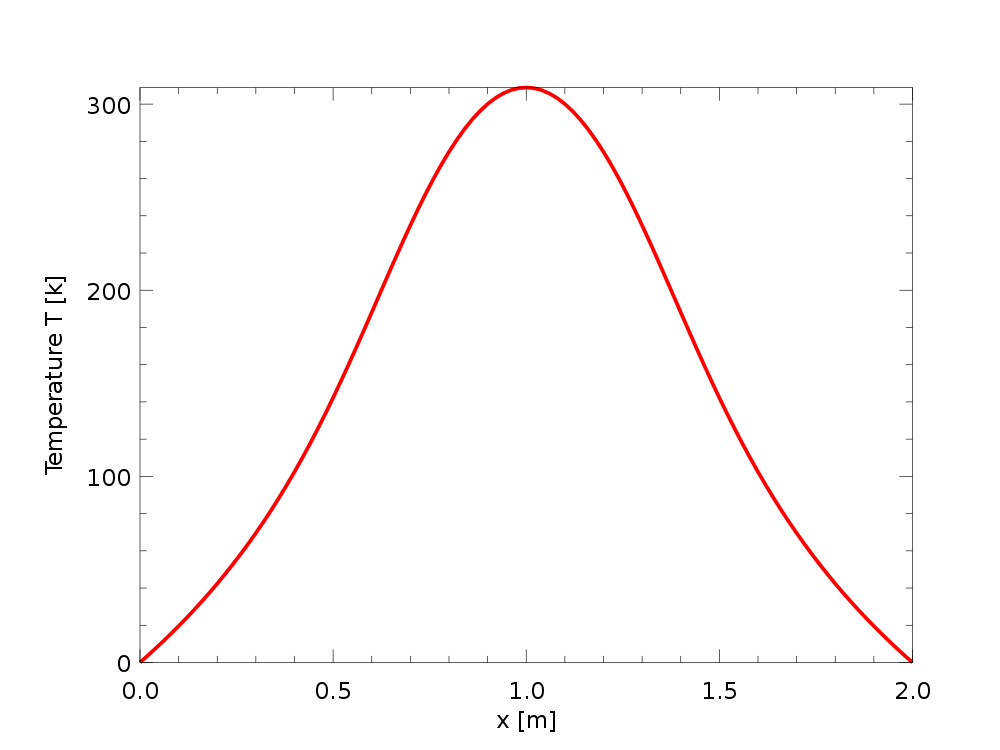
\includegraphics[width=\columnwidth]{regsolution.png}
\footnotesize{\caption{Heat Equation solution with \emph{k}(\emph{T})}}
\end{figure}
\begin{figure}
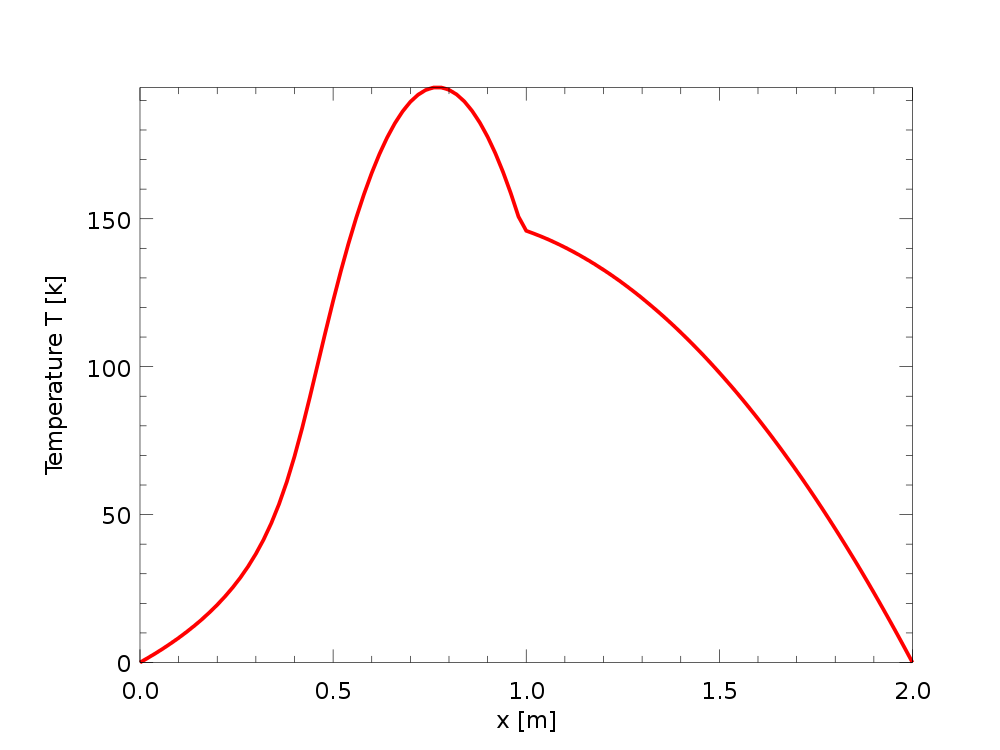
\includegraphics[width=\columnwidth]{discontheat.png}
\footnotesize{\caption{Solution with discontinuous \emph{k}}}
\end{figure}
\section*{Implementation}
Boundary conditions were moved to a seperate module in order to easily update all boundary conditions at once. In addition, the evaluation of \emph{k}
was also moved to this module; allowing for conductivity models to be implemented easily. Picard Iteration proved adequate, converging
in 14 iterations for the test case.
\section*{Discontinous Conductivity}
The modular structure of the code easily lends itself to arbitrary specification of \emph{k}
\[k = 
\begin{cases}
k_0 + k_1 e^{\frac{T}{T_0}} & x \leq 1 \\
k_3 & x > 1
\end{cases}\]
\begin{figure}
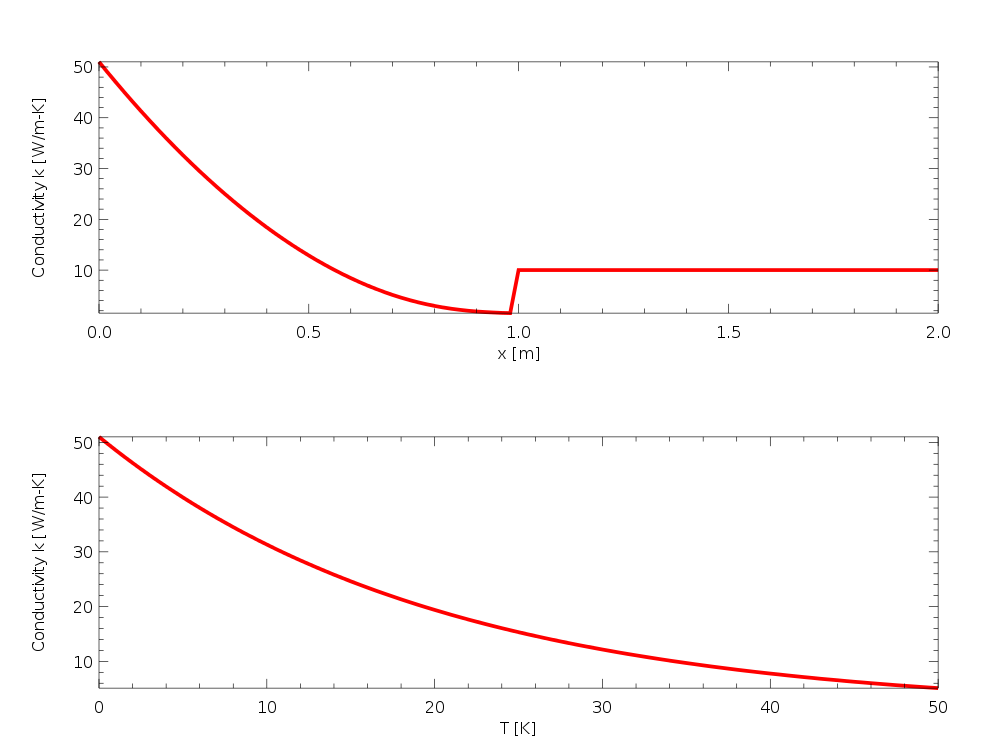
\includegraphics[width=\columnwidth]{conductivity.png}
\footnotesize{\caption{Discontinuous \emph{k}(\emph{x},\emph{T}) conductivity $\frac{k_1}{k_0}=20;\hspace{1em} k_3=10$}}
\end{figure}
Notably, the required number of iterations over the continuous model increased depending on $\frac{k_1}{k_0}$. A model with discontinuous
\emph{k} could model fuel rods in an enclosure or a heating element where the thermal conductivity is a strong function of temperature.

\section*{Performance Improvement}
A better performing non-linear solver could be achieved by using a higher order method such as Halley's Method.
\[x_{n+1} = x_n - \frac{2 f(x_n)f'(x_n)}{2f'(x_n)^2-f(x_n)f''(x_n)}\]
\[(2J^2-J'f(x_n))\Delta x = - 2Jf(x_n)\]
Using numerical derivation, the Jacobian and derivative of the Jacobian could be constructed with ease.
The convergence would be greater than Newton's Method, but the extra overhead would only be worthwhile on
very non-linear problems.
\begin{figure}
\begin{center}
\begin{tabular}{|l|c|r|}
\hline
$\frac{k_1}{k_0}$ & Discontinuous & Continuous\\ \hline
10 & 16 & 15\\ \hline
25 & 24 & 17\\ \hline
50 & 27 & 14\\ \hline
75 & 19 & 9\\ \hline
100 & 13 & 8\\ \hline
150 & 9 & 6\\ \hline
200 & 7 & 6\\ \hline
\end{tabular}
\end{center}
\footnotesize{\caption{Conductivity Model Performance}}
\end{figure}
\end{document}
